% =====================================================================
%  kap5_pengestroemme.tex  —  slide redraw of fig:kap5_pengestroemme
%  Source of truth: notes ch.5 "5 Realkredit.tex", figur pengestrømme.
%
%  Slide-optimised redraw (paper-density stripped, labels enlarged,
%  institut tinted in brand teal). Built in phases so the arrows can be
%  revealed one flow at a time on the slide (reveal.js fragment stack):
%     \phase = 1  ->  origination only  (money flows IN to fund the loan)
%     \phase = 2  ->  full              (+ servicing flows over the life)
%
%  Build (from slides_side/src/images/_tikz_src/):
%     pdflatex "\def\phase{1}% =====================================================================
%  kap5_pengestroemme.tex  —  slide redraw of fig:kap5_pengestroemme
%  Source of truth: notes ch.5 "5 Realkredit.tex", figur pengestrømme.
%
%  Slide-optimised redraw (paper-density stripped, labels enlarged,
%  institut tinted in brand teal). Built in phases so the arrows can be
%  revealed one flow at a time on the slide (reveal.js fragment stack):
%     \phase = 1  ->  origination only  (money flows IN to fund the loan)
%     \phase = 2  ->  full              (+ servicing flows over the life)
%
%  Build (from slides_side/src/images/_tikz_src/):
%     pdflatex "\def\phase{1}% =====================================================================
%  kap5_pengestroemme.tex  —  slide redraw of fig:kap5_pengestroemme
%  Source of truth: notes ch.5 "5 Realkredit.tex", figur pengestrømme.
%
%  Slide-optimised redraw (paper-density stripped, labels enlarged,
%  institut tinted in brand teal). Built in phases so the arrows can be
%  revealed one flow at a time on the slide (reveal.js fragment stack):
%     \phase = 1  ->  origination only  (money flows IN to fund the loan)
%     \phase = 2  ->  full              (+ servicing flows over the life)
%
%  Build (from slides_side/src/images/_tikz_src/):
%     pdflatex "\def\phase{1}% =====================================================================
%  kap5_pengestroemme.tex  —  slide redraw of fig:kap5_pengestroemme
%  Source of truth: notes ch.5 "5 Realkredit.tex", figur pengestrømme.
%
%  Slide-optimised redraw (paper-density stripped, labels enlarged,
%  institut tinted in brand teal). Built in phases so the arrows can be
%  revealed one flow at a time on the slide (reveal.js fragment stack):
%     \phase = 1  ->  origination only  (money flows IN to fund the loan)
%     \phase = 2  ->  full              (+ servicing flows over the life)
%
%  Build (from slides_side/src/images/_tikz_src/):
%     pdflatex "\def\phase{1}\input{kap5_pengestroemme.tex}"  (rename out)
%     pdflatex "\def\phase{2}\input{kap5_pengestroemme.tex}"
%  then dvisvgm --pdf on each. See build_tikz.sh in this folder.
% =====================================================================
\providecommand{\phase}{2}      % default: full figure
\documentclass[border=6pt]{standalone}
\usepackage[T1]{fontenc}
\usepackage[utf8]{inputenc}
\usepackage[scaled=0.98]{helvet}
\renewcommand{\familydefault}{\sfdefault}
\usepackage{tikz}
\usetikzlibrary{arrows.meta, positioning, calc}

\definecolor{brandteal}{HTML}{045D5D}
\definecolor{brandgold}{HTML}{C9A227} % muted gold (readable on white)
\definecolor{flowin}{HTML}{1F6FB2}    % origination flow (blue)
\definecolor{flowout}{HTML}{045D5D}   % servicing flow (teal)

\begin{document}
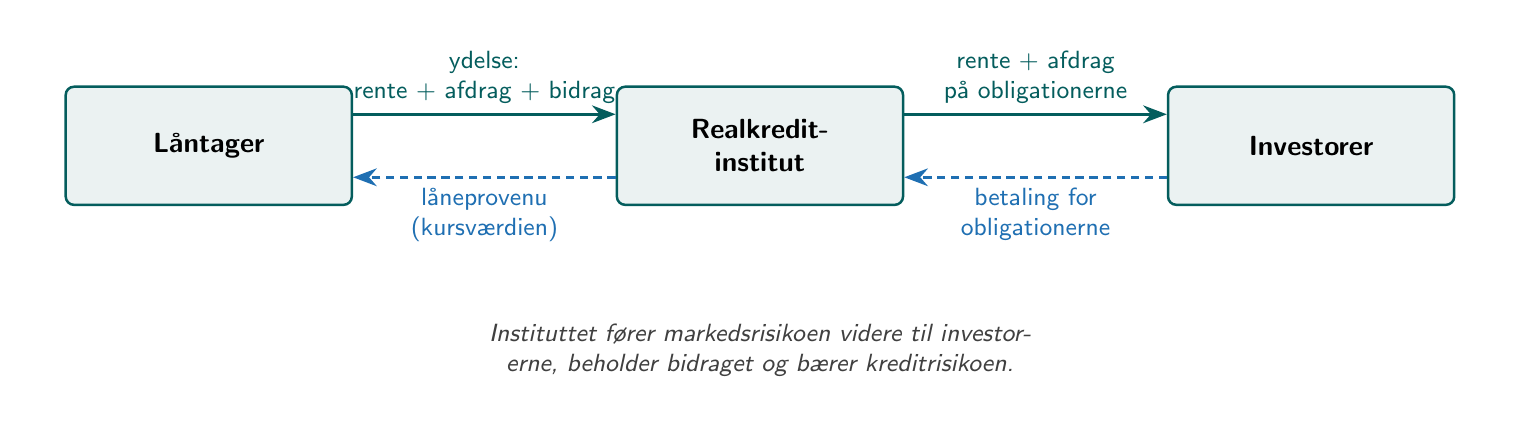
\begin{tikzpicture}[
    part/.style   = {draw=brandteal, line width=0.9pt, rounded corners=3pt,
                     fill=brandteal!8, align=center, minimum height=15mm,
                     text width=34mm, font=\normalsize\bfseries},
    lblup/.style  = {font=\small, align=center, text width=38mm, text=flowout},
    lbldn/.style  = {font=\small, align=center, text width=38mm, text=flowin},
    servicing/.style = {-{Stealth[length=3mm]}, line width=1.1pt, flowout},
    origin/.style    = {-{Stealth[length=3mm]}, line width=1.1pt, flowin, densely dashed},
]

% Fixed canvas so every phase exports at identical size -> the reveal.js
% fragment-stack animates without the boxes jumping between steps.
\useasboundingbox (-2.3,-3.4) rectangle (16.3,1.5);

% --- the three parties -------------------------------------------------
\node[part] (laantager) at (0,0)   {Låntager};
\node[part] (institut)  at (7,0)   {Realkredit-\\institut};
\node[part] (investor)  at (14,0)  {Investorer};

% --- phase 1: origination (money flows in, bottom arrows) --------------
\ifnum\phase>0
  \draw[origin] ([yshift=-4mm]investor.west) --
        node[lbldn, below] {betaling for\\obligationerne}
        ([yshift=-4mm]institut.east);
  \draw[origin] ([yshift=-4mm]institut.west) --
        node[lbldn, below] {låneprovenu\\(kursværdien)}
        ([yshift=-4mm]laantager.east);
\fi

% --- phase 2: servicing (life of the loan, top arrows) ----------------
\ifnum\phase>1
  \draw[servicing] ([yshift=4mm]laantager.east) --
        node[lblup, above] {ydelse:\\rente + afdrag + bidrag}
        ([yshift=4mm]institut.west);
  \draw[servicing] ([yshift=4mm]institut.east) --
        node[lblup, above] {rente + afdrag\\på obligationerne}
        ([yshift=4mm]investor.west);
  \node[align=center, font=\small\itshape, text width=105mm, text=black!75]
        at (7,-2.6)
        {Instituttet fører markedsrisikoen videre til investorerne,
         beholder bidraget og bærer kreditrisikoen.};
\fi

\end{tikzpicture}
\end{document}
"  (rename out)
%     pdflatex "\def\phase{2}% =====================================================================
%  kap5_pengestroemme.tex  —  slide redraw of fig:kap5_pengestroemme
%  Source of truth: notes ch.5 "5 Realkredit.tex", figur pengestrømme.
%
%  Slide-optimised redraw (paper-density stripped, labels enlarged,
%  institut tinted in brand teal). Built in phases so the arrows can be
%  revealed one flow at a time on the slide (reveal.js fragment stack):
%     \phase = 1  ->  origination only  (money flows IN to fund the loan)
%     \phase = 2  ->  full              (+ servicing flows over the life)
%
%  Build (from slides_side/src/images/_tikz_src/):
%     pdflatex "\def\phase{1}\input{kap5_pengestroemme.tex}"  (rename out)
%     pdflatex "\def\phase{2}\input{kap5_pengestroemme.tex}"
%  then dvisvgm --pdf on each. See build_tikz.sh in this folder.
% =====================================================================
\providecommand{\phase}{2}      % default: full figure
\documentclass[border=6pt]{standalone}
\usepackage[T1]{fontenc}
\usepackage[utf8]{inputenc}
\usepackage[scaled=0.98]{helvet}
\renewcommand{\familydefault}{\sfdefault}
\usepackage{tikz}
\usetikzlibrary{arrows.meta, positioning, calc}

\definecolor{brandteal}{HTML}{045D5D}
\definecolor{brandgold}{HTML}{C9A227} % muted gold (readable on white)
\definecolor{flowin}{HTML}{1F6FB2}    % origination flow (blue)
\definecolor{flowout}{HTML}{045D5D}   % servicing flow (teal)

\begin{document}
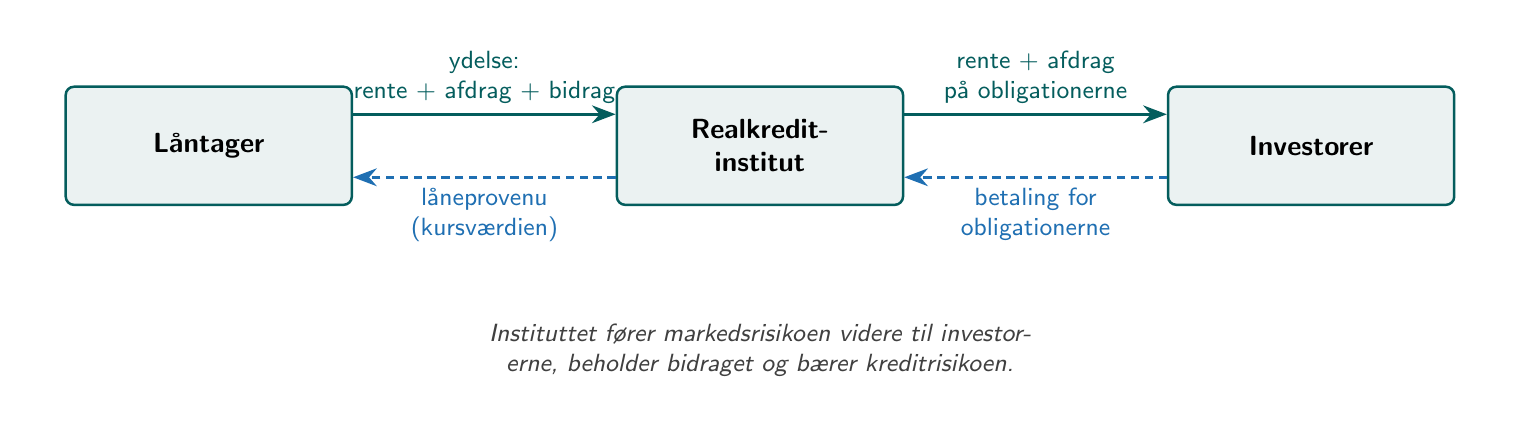
\begin{tikzpicture}[
    part/.style   = {draw=brandteal, line width=0.9pt, rounded corners=3pt,
                     fill=brandteal!8, align=center, minimum height=15mm,
                     text width=34mm, font=\normalsize\bfseries},
    lblup/.style  = {font=\small, align=center, text width=38mm, text=flowout},
    lbldn/.style  = {font=\small, align=center, text width=38mm, text=flowin},
    servicing/.style = {-{Stealth[length=3mm]}, line width=1.1pt, flowout},
    origin/.style    = {-{Stealth[length=3mm]}, line width=1.1pt, flowin, densely dashed},
]

% Fixed canvas so every phase exports at identical size -> the reveal.js
% fragment-stack animates without the boxes jumping between steps.
\useasboundingbox (-2.3,-3.4) rectangle (16.3,1.5);

% --- the three parties -------------------------------------------------
\node[part] (laantager) at (0,0)   {Låntager};
\node[part] (institut)  at (7,0)   {Realkredit-\\institut};
\node[part] (investor)  at (14,0)  {Investorer};

% --- phase 1: origination (money flows in, bottom arrows) --------------
\ifnum\phase>0
  \draw[origin] ([yshift=-4mm]investor.west) --
        node[lbldn, below] {betaling for\\obligationerne}
        ([yshift=-4mm]institut.east);
  \draw[origin] ([yshift=-4mm]institut.west) --
        node[lbldn, below] {låneprovenu\\(kursværdien)}
        ([yshift=-4mm]laantager.east);
\fi

% --- phase 2: servicing (life of the loan, top arrows) ----------------
\ifnum\phase>1
  \draw[servicing] ([yshift=4mm]laantager.east) --
        node[lblup, above] {ydelse:\\rente + afdrag + bidrag}
        ([yshift=4mm]institut.west);
  \draw[servicing] ([yshift=4mm]institut.east) --
        node[lblup, above] {rente + afdrag\\på obligationerne}
        ([yshift=4mm]investor.west);
  \node[align=center, font=\small\itshape, text width=105mm, text=black!75]
        at (7,-2.6)
        {Instituttet fører markedsrisikoen videre til investorerne,
         beholder bidraget og bærer kreditrisikoen.};
\fi

\end{tikzpicture}
\end{document}
"
%  then dvisvgm --pdf on each. See build_tikz.sh in this folder.
% =====================================================================
\providecommand{\phase}{2}      % default: full figure
\documentclass[border=6pt]{standalone}
\usepackage[T1]{fontenc}
\usepackage[utf8]{inputenc}
\usepackage[scaled=0.98]{helvet}
\renewcommand{\familydefault}{\sfdefault}
\usepackage{tikz}
\usetikzlibrary{arrows.meta, positioning, calc}

\definecolor{brandteal}{HTML}{045D5D}
\definecolor{brandgold}{HTML}{C9A227} % muted gold (readable on white)
\definecolor{flowin}{HTML}{1F6FB2}    % origination flow (blue)
\definecolor{flowout}{HTML}{045D5D}   % servicing flow (teal)

\begin{document}
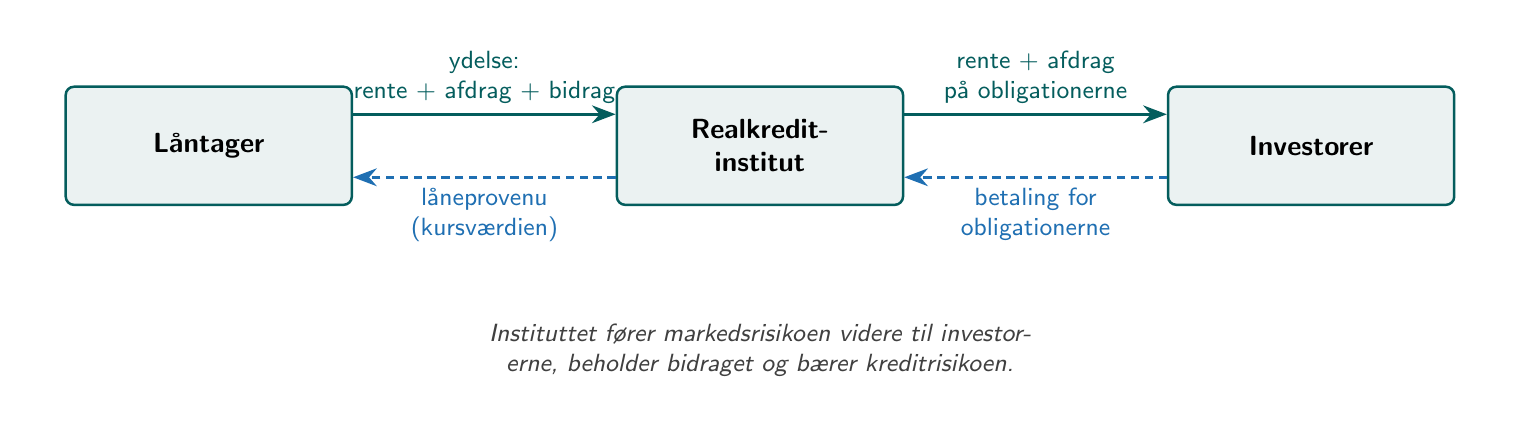
\begin{tikzpicture}[
    part/.style   = {draw=brandteal, line width=0.9pt, rounded corners=3pt,
                     fill=brandteal!8, align=center, minimum height=15mm,
                     text width=34mm, font=\normalsize\bfseries},
    lblup/.style  = {font=\small, align=center, text width=38mm, text=flowout},
    lbldn/.style  = {font=\small, align=center, text width=38mm, text=flowin},
    servicing/.style = {-{Stealth[length=3mm]}, line width=1.1pt, flowout},
    origin/.style    = {-{Stealth[length=3mm]}, line width=1.1pt, flowin, densely dashed},
]

% Fixed canvas so every phase exports at identical size -> the reveal.js
% fragment-stack animates without the boxes jumping between steps.
\useasboundingbox (-2.3,-3.4) rectangle (16.3,1.5);

% --- the three parties -------------------------------------------------
\node[part] (laantager) at (0,0)   {Låntager};
\node[part] (institut)  at (7,0)   {Realkredit-\\institut};
\node[part] (investor)  at (14,0)  {Investorer};

% --- phase 1: origination (money flows in, bottom arrows) --------------
\ifnum\phase>0
  \draw[origin] ([yshift=-4mm]investor.west) --
        node[lbldn, below] {betaling for\\obligationerne}
        ([yshift=-4mm]institut.east);
  \draw[origin] ([yshift=-4mm]institut.west) --
        node[lbldn, below] {låneprovenu\\(kursværdien)}
        ([yshift=-4mm]laantager.east);
\fi

% --- phase 2: servicing (life of the loan, top arrows) ----------------
\ifnum\phase>1
  \draw[servicing] ([yshift=4mm]laantager.east) --
        node[lblup, above] {ydelse:\\rente + afdrag + bidrag}
        ([yshift=4mm]institut.west);
  \draw[servicing] ([yshift=4mm]institut.east) --
        node[lblup, above] {rente + afdrag\\på obligationerne}
        ([yshift=4mm]investor.west);
  \node[align=center, font=\small\itshape, text width=105mm, text=black!75]
        at (7,-2.6)
        {Instituttet fører markedsrisikoen videre til investorerne,
         beholder bidraget og bærer kreditrisikoen.};
\fi

\end{tikzpicture}
\end{document}
"  (rename out)
%     pdflatex "\def\phase{2}% =====================================================================
%  kap5_pengestroemme.tex  —  slide redraw of fig:kap5_pengestroemme
%  Source of truth: notes ch.5 "5 Realkredit.tex", figur pengestrømme.
%
%  Slide-optimised redraw (paper-density stripped, labels enlarged,
%  institut tinted in brand teal). Built in phases so the arrows can be
%  revealed one flow at a time on the slide (reveal.js fragment stack):
%     \phase = 1  ->  origination only  (money flows IN to fund the loan)
%     \phase = 2  ->  full              (+ servicing flows over the life)
%
%  Build (from slides_side/src/images/_tikz_src/):
%     pdflatex "\def\phase{1}% =====================================================================
%  kap5_pengestroemme.tex  —  slide redraw of fig:kap5_pengestroemme
%  Source of truth: notes ch.5 "5 Realkredit.tex", figur pengestrømme.
%
%  Slide-optimised redraw (paper-density stripped, labels enlarged,
%  institut tinted in brand teal). Built in phases so the arrows can be
%  revealed one flow at a time on the slide (reveal.js fragment stack):
%     \phase = 1  ->  origination only  (money flows IN to fund the loan)
%     \phase = 2  ->  full              (+ servicing flows over the life)
%
%  Build (from slides_side/src/images/_tikz_src/):
%     pdflatex "\def\phase{1}\input{kap5_pengestroemme.tex}"  (rename out)
%     pdflatex "\def\phase{2}\input{kap5_pengestroemme.tex}"
%  then dvisvgm --pdf on each. See build_tikz.sh in this folder.
% =====================================================================
\providecommand{\phase}{2}      % default: full figure
\documentclass[border=6pt]{standalone}
\usepackage[T1]{fontenc}
\usepackage[utf8]{inputenc}
\usepackage[scaled=0.98]{helvet}
\renewcommand{\familydefault}{\sfdefault}
\usepackage{tikz}
\usetikzlibrary{arrows.meta, positioning, calc}

\definecolor{brandteal}{HTML}{045D5D}
\definecolor{brandgold}{HTML}{C9A227} % muted gold (readable on white)
\definecolor{flowin}{HTML}{1F6FB2}    % origination flow (blue)
\definecolor{flowout}{HTML}{045D5D}   % servicing flow (teal)

\begin{document}
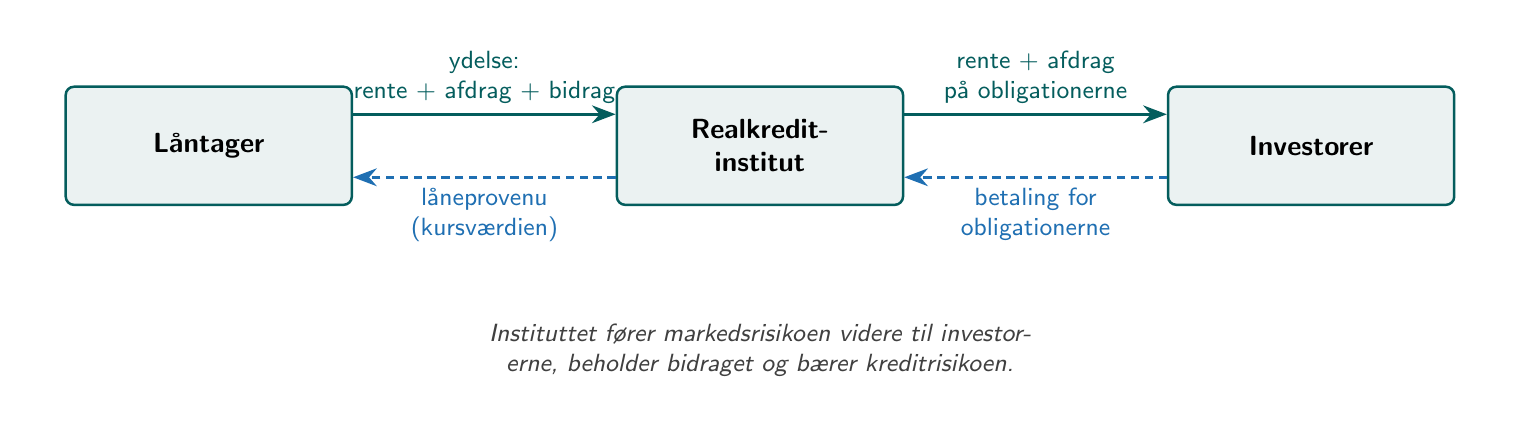
\begin{tikzpicture}[
    part/.style   = {draw=brandteal, line width=0.9pt, rounded corners=3pt,
                     fill=brandteal!8, align=center, minimum height=15mm,
                     text width=34mm, font=\normalsize\bfseries},
    lblup/.style  = {font=\small, align=center, text width=38mm, text=flowout},
    lbldn/.style  = {font=\small, align=center, text width=38mm, text=flowin},
    servicing/.style = {-{Stealth[length=3mm]}, line width=1.1pt, flowout},
    origin/.style    = {-{Stealth[length=3mm]}, line width=1.1pt, flowin, densely dashed},
]

% Fixed canvas so every phase exports at identical size -> the reveal.js
% fragment-stack animates without the boxes jumping between steps.
\useasboundingbox (-2.3,-3.4) rectangle (16.3,1.5);

% --- the three parties -------------------------------------------------
\node[part] (laantager) at (0,0)   {Låntager};
\node[part] (institut)  at (7,0)   {Realkredit-\\institut};
\node[part] (investor)  at (14,0)  {Investorer};

% --- phase 1: origination (money flows in, bottom arrows) --------------
\ifnum\phase>0
  \draw[origin] ([yshift=-4mm]investor.west) --
        node[lbldn, below] {betaling for\\obligationerne}
        ([yshift=-4mm]institut.east);
  \draw[origin] ([yshift=-4mm]institut.west) --
        node[lbldn, below] {låneprovenu\\(kursværdien)}
        ([yshift=-4mm]laantager.east);
\fi

% --- phase 2: servicing (life of the loan, top arrows) ----------------
\ifnum\phase>1
  \draw[servicing] ([yshift=4mm]laantager.east) --
        node[lblup, above] {ydelse:\\rente + afdrag + bidrag}
        ([yshift=4mm]institut.west);
  \draw[servicing] ([yshift=4mm]institut.east) --
        node[lblup, above] {rente + afdrag\\på obligationerne}
        ([yshift=4mm]investor.west);
  \node[align=center, font=\small\itshape, text width=105mm, text=black!75]
        at (7,-2.6)
        {Instituttet fører markedsrisikoen videre til investorerne,
         beholder bidraget og bærer kreditrisikoen.};
\fi

\end{tikzpicture}
\end{document}
"  (rename out)
%     pdflatex "\def\phase{2}% =====================================================================
%  kap5_pengestroemme.tex  —  slide redraw of fig:kap5_pengestroemme
%  Source of truth: notes ch.5 "5 Realkredit.tex", figur pengestrømme.
%
%  Slide-optimised redraw (paper-density stripped, labels enlarged,
%  institut tinted in brand teal). Built in phases so the arrows can be
%  revealed one flow at a time on the slide (reveal.js fragment stack):
%     \phase = 1  ->  origination only  (money flows IN to fund the loan)
%     \phase = 2  ->  full              (+ servicing flows over the life)
%
%  Build (from slides_side/src/images/_tikz_src/):
%     pdflatex "\def\phase{1}\input{kap5_pengestroemme.tex}"  (rename out)
%     pdflatex "\def\phase{2}\input{kap5_pengestroemme.tex}"
%  then dvisvgm --pdf on each. See build_tikz.sh in this folder.
% =====================================================================
\providecommand{\phase}{2}      % default: full figure
\documentclass[border=6pt]{standalone}
\usepackage[T1]{fontenc}
\usepackage[utf8]{inputenc}
\usepackage[scaled=0.98]{helvet}
\renewcommand{\familydefault}{\sfdefault}
\usepackage{tikz}
\usetikzlibrary{arrows.meta, positioning, calc}

\definecolor{brandteal}{HTML}{045D5D}
\definecolor{brandgold}{HTML}{C9A227} % muted gold (readable on white)
\definecolor{flowin}{HTML}{1F6FB2}    % origination flow (blue)
\definecolor{flowout}{HTML}{045D5D}   % servicing flow (teal)

\begin{document}
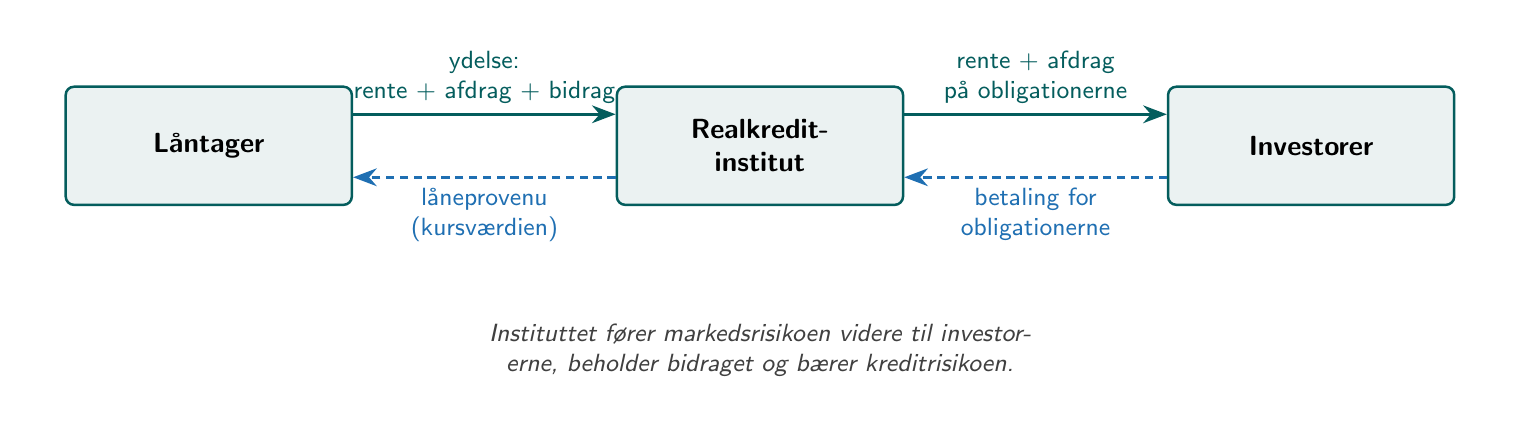
\begin{tikzpicture}[
    part/.style   = {draw=brandteal, line width=0.9pt, rounded corners=3pt,
                     fill=brandteal!8, align=center, minimum height=15mm,
                     text width=34mm, font=\normalsize\bfseries},
    lblup/.style  = {font=\small, align=center, text width=38mm, text=flowout},
    lbldn/.style  = {font=\small, align=center, text width=38mm, text=flowin},
    servicing/.style = {-{Stealth[length=3mm]}, line width=1.1pt, flowout},
    origin/.style    = {-{Stealth[length=3mm]}, line width=1.1pt, flowin, densely dashed},
]

% Fixed canvas so every phase exports at identical size -> the reveal.js
% fragment-stack animates without the boxes jumping between steps.
\useasboundingbox (-2.3,-3.4) rectangle (16.3,1.5);

% --- the three parties -------------------------------------------------
\node[part] (laantager) at (0,0)   {Låntager};
\node[part] (institut)  at (7,0)   {Realkredit-\\institut};
\node[part] (investor)  at (14,0)  {Investorer};

% --- phase 1: origination (money flows in, bottom arrows) --------------
\ifnum\phase>0
  \draw[origin] ([yshift=-4mm]investor.west) --
        node[lbldn, below] {betaling for\\obligationerne}
        ([yshift=-4mm]institut.east);
  \draw[origin] ([yshift=-4mm]institut.west) --
        node[lbldn, below] {låneprovenu\\(kursværdien)}
        ([yshift=-4mm]laantager.east);
\fi

% --- phase 2: servicing (life of the loan, top arrows) ----------------
\ifnum\phase>1
  \draw[servicing] ([yshift=4mm]laantager.east) --
        node[lblup, above] {ydelse:\\rente + afdrag + bidrag}
        ([yshift=4mm]institut.west);
  \draw[servicing] ([yshift=4mm]institut.east) --
        node[lblup, above] {rente + afdrag\\på obligationerne}
        ([yshift=4mm]investor.west);
  \node[align=center, font=\small\itshape, text width=105mm, text=black!75]
        at (7,-2.6)
        {Instituttet fører markedsrisikoen videre til investorerne,
         beholder bidraget og bærer kreditrisikoen.};
\fi

\end{tikzpicture}
\end{document}
"
%  then dvisvgm --pdf on each. See build_tikz.sh in this folder.
% =====================================================================
\providecommand{\phase}{2}      % default: full figure
\documentclass[border=6pt]{standalone}
\usepackage[T1]{fontenc}
\usepackage[utf8]{inputenc}
\usepackage[scaled=0.98]{helvet}
\renewcommand{\familydefault}{\sfdefault}
\usepackage{tikz}
\usetikzlibrary{arrows.meta, positioning, calc}

\definecolor{brandteal}{HTML}{045D5D}
\definecolor{brandgold}{HTML}{C9A227} % muted gold (readable on white)
\definecolor{flowin}{HTML}{1F6FB2}    % origination flow (blue)
\definecolor{flowout}{HTML}{045D5D}   % servicing flow (teal)

\begin{document}
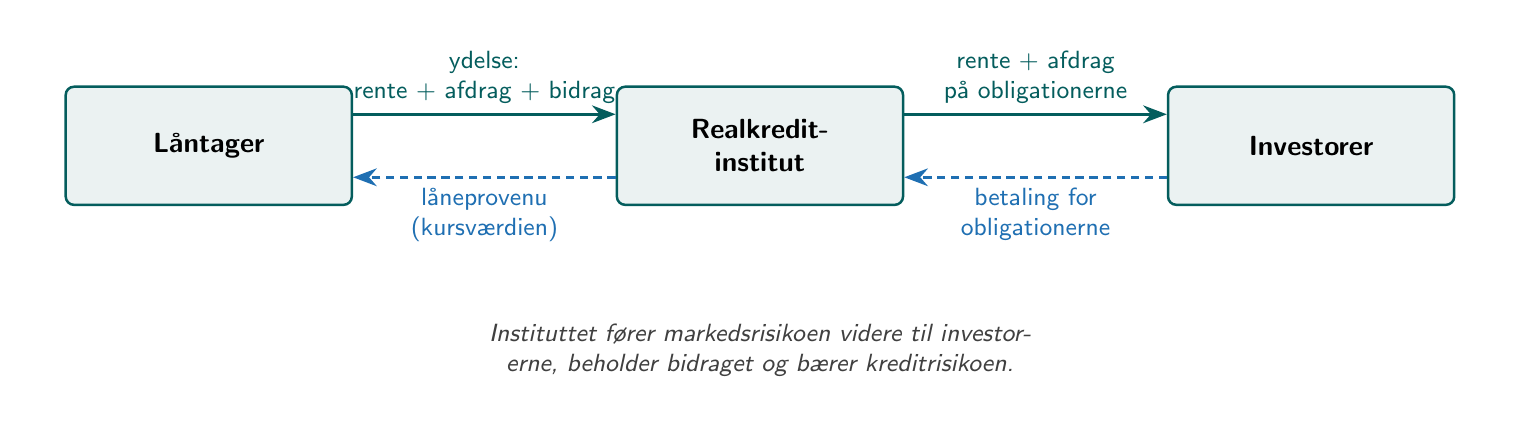
\begin{tikzpicture}[
    part/.style   = {draw=brandteal, line width=0.9pt, rounded corners=3pt,
                     fill=brandteal!8, align=center, minimum height=15mm,
                     text width=34mm, font=\normalsize\bfseries},
    lblup/.style  = {font=\small, align=center, text width=38mm, text=flowout},
    lbldn/.style  = {font=\small, align=center, text width=38mm, text=flowin},
    servicing/.style = {-{Stealth[length=3mm]}, line width=1.1pt, flowout},
    origin/.style    = {-{Stealth[length=3mm]}, line width=1.1pt, flowin, densely dashed},
]

% Fixed canvas so every phase exports at identical size -> the reveal.js
% fragment-stack animates without the boxes jumping between steps.
\useasboundingbox (-2.3,-3.4) rectangle (16.3,1.5);

% --- the three parties -------------------------------------------------
\node[part] (laantager) at (0,0)   {Låntager};
\node[part] (institut)  at (7,0)   {Realkredit-\\institut};
\node[part] (investor)  at (14,0)  {Investorer};

% --- phase 1: origination (money flows in, bottom arrows) --------------
\ifnum\phase>0
  \draw[origin] ([yshift=-4mm]investor.west) --
        node[lbldn, below] {betaling for\\obligationerne}
        ([yshift=-4mm]institut.east);
  \draw[origin] ([yshift=-4mm]institut.west) --
        node[lbldn, below] {låneprovenu\\(kursværdien)}
        ([yshift=-4mm]laantager.east);
\fi

% --- phase 2: servicing (life of the loan, top arrows) ----------------
\ifnum\phase>1
  \draw[servicing] ([yshift=4mm]laantager.east) --
        node[lblup, above] {ydelse:\\rente + afdrag + bidrag}
        ([yshift=4mm]institut.west);
  \draw[servicing] ([yshift=4mm]institut.east) --
        node[lblup, above] {rente + afdrag\\på obligationerne}
        ([yshift=4mm]investor.west);
  \node[align=center, font=\small\itshape, text width=105mm, text=black!75]
        at (7,-2.6)
        {Instituttet fører markedsrisikoen videre til investorerne,
         beholder bidraget og bærer kreditrisikoen.};
\fi

\end{tikzpicture}
\end{document}
"
%  then dvisvgm --pdf on each. See build_tikz.sh in this folder.
% =====================================================================
\providecommand{\phase}{2}      % default: full figure
\documentclass[border=6pt]{standalone}
\usepackage[T1]{fontenc}
\usepackage[utf8]{inputenc}
\usepackage[scaled=0.98]{helvet}
\renewcommand{\familydefault}{\sfdefault}
\usepackage{tikz}
\usetikzlibrary{arrows.meta, positioning, calc}

\definecolor{brandteal}{HTML}{045D5D}
\definecolor{brandgold}{HTML}{C9A227} % muted gold (readable on white)
\definecolor{flowin}{HTML}{1F6FB2}    % origination flow (blue)
\definecolor{flowout}{HTML}{045D5D}   % servicing flow (teal)

\begin{document}
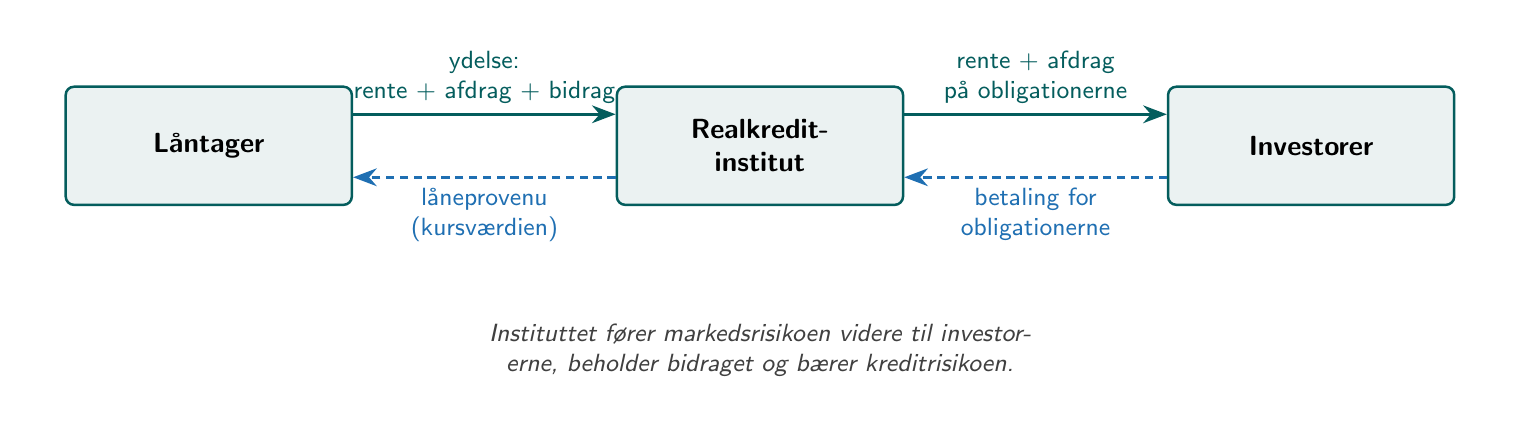
\begin{tikzpicture}[
    part/.style   = {draw=brandteal, line width=0.9pt, rounded corners=3pt,
                     fill=brandteal!8, align=center, minimum height=15mm,
                     text width=34mm, font=\normalsize\bfseries},
    lblup/.style  = {font=\small, align=center, text width=38mm, text=flowout},
    lbldn/.style  = {font=\small, align=center, text width=38mm, text=flowin},
    servicing/.style = {-{Stealth[length=3mm]}, line width=1.1pt, flowout},
    origin/.style    = {-{Stealth[length=3mm]}, line width=1.1pt, flowin, densely dashed},
]

% Fixed canvas so every phase exports at identical size -> the reveal.js
% fragment-stack animates without the boxes jumping between steps.
\useasboundingbox (-2.3,-3.4) rectangle (16.3,1.5);

% --- the three parties -------------------------------------------------
\node[part] (laantager) at (0,0)   {Låntager};
\node[part] (institut)  at (7,0)   {Realkredit-\\institut};
\node[part] (investor)  at (14,0)  {Investorer};

% --- phase 1: origination (money flows in, bottom arrows) --------------
\ifnum\phase>0
  \draw[origin] ([yshift=-4mm]investor.west) --
        node[lbldn, below] {betaling for\\obligationerne}
        ([yshift=-4mm]institut.east);
  \draw[origin] ([yshift=-4mm]institut.west) --
        node[lbldn, below] {låneprovenu\\(kursværdien)}
        ([yshift=-4mm]laantager.east);
\fi

% --- phase 2: servicing (life of the loan, top arrows) ----------------
\ifnum\phase>1
  \draw[servicing] ([yshift=4mm]laantager.east) --
        node[lblup, above] {ydelse:\\rente + afdrag + bidrag}
        ([yshift=4mm]institut.west);
  \draw[servicing] ([yshift=4mm]institut.east) --
        node[lblup, above] {rente + afdrag\\på obligationerne}
        ([yshift=4mm]investor.west);
  \node[align=center, font=\small\itshape, text width=105mm, text=black!75]
        at (7,-2.6)
        {Instituttet fører markedsrisikoen videre til investorerne,
         beholder bidraget og bærer kreditrisikoen.};
\fi

\end{tikzpicture}
\end{document}
"  (rename out)
%     pdflatex "\def\phase{2}% =====================================================================
%  kap5_pengestroemme.tex  —  slide redraw of fig:kap5_pengestroemme
%  Source of truth: notes ch.5 "5 Realkredit.tex", figur pengestrømme.
%
%  Slide-optimised redraw (paper-density stripped, labels enlarged,
%  institut tinted in brand teal). Built in phases so the arrows can be
%  revealed one flow at a time on the slide (reveal.js fragment stack):
%     \phase = 1  ->  origination only  (money flows IN to fund the loan)
%     \phase = 2  ->  full              (+ servicing flows over the life)
%
%  Build (from slides_side/src/images/_tikz_src/):
%     pdflatex "\def\phase{1}% =====================================================================
%  kap5_pengestroemme.tex  —  slide redraw of fig:kap5_pengestroemme
%  Source of truth: notes ch.5 "5 Realkredit.tex", figur pengestrømme.
%
%  Slide-optimised redraw (paper-density stripped, labels enlarged,
%  institut tinted in brand teal). Built in phases so the arrows can be
%  revealed one flow at a time on the slide (reveal.js fragment stack):
%     \phase = 1  ->  origination only  (money flows IN to fund the loan)
%     \phase = 2  ->  full              (+ servicing flows over the life)
%
%  Build (from slides_side/src/images/_tikz_src/):
%     pdflatex "\def\phase{1}% =====================================================================
%  kap5_pengestroemme.tex  —  slide redraw of fig:kap5_pengestroemme
%  Source of truth: notes ch.5 "5 Realkredit.tex", figur pengestrømme.
%
%  Slide-optimised redraw (paper-density stripped, labels enlarged,
%  institut tinted in brand teal). Built in phases so the arrows can be
%  revealed one flow at a time on the slide (reveal.js fragment stack):
%     \phase = 1  ->  origination only  (money flows IN to fund the loan)
%     \phase = 2  ->  full              (+ servicing flows over the life)
%
%  Build (from slides_side/src/images/_tikz_src/):
%     pdflatex "\def\phase{1}\input{kap5_pengestroemme.tex}"  (rename out)
%     pdflatex "\def\phase{2}\input{kap5_pengestroemme.tex}"
%  then dvisvgm --pdf on each. See build_tikz.sh in this folder.
% =====================================================================
\providecommand{\phase}{2}      % default: full figure
\documentclass[border=6pt]{standalone}
\usepackage[T1]{fontenc}
\usepackage[utf8]{inputenc}
\usepackage[scaled=0.98]{helvet}
\renewcommand{\familydefault}{\sfdefault}
\usepackage{tikz}
\usetikzlibrary{arrows.meta, positioning, calc}

\definecolor{brandteal}{HTML}{045D5D}
\definecolor{brandgold}{HTML}{C9A227} % muted gold (readable on white)
\definecolor{flowin}{HTML}{1F6FB2}    % origination flow (blue)
\definecolor{flowout}{HTML}{045D5D}   % servicing flow (teal)

\begin{document}
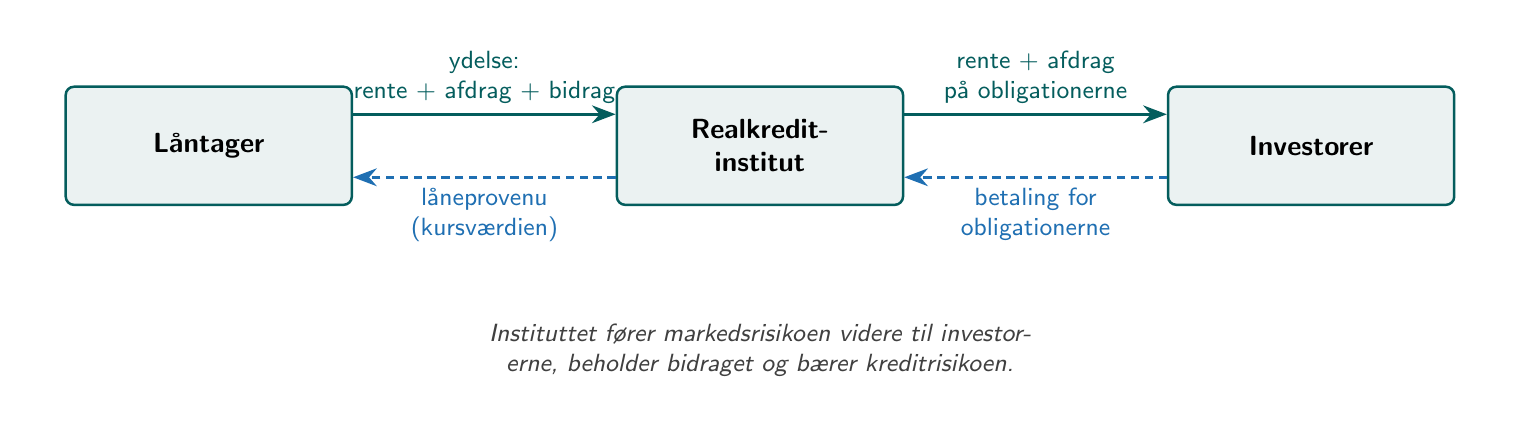
\begin{tikzpicture}[
    part/.style   = {draw=brandteal, line width=0.9pt, rounded corners=3pt,
                     fill=brandteal!8, align=center, minimum height=15mm,
                     text width=34mm, font=\normalsize\bfseries},
    lblup/.style  = {font=\small, align=center, text width=38mm, text=flowout},
    lbldn/.style  = {font=\small, align=center, text width=38mm, text=flowin},
    servicing/.style = {-{Stealth[length=3mm]}, line width=1.1pt, flowout},
    origin/.style    = {-{Stealth[length=3mm]}, line width=1.1pt, flowin, densely dashed},
]

% Fixed canvas so every phase exports at identical size -> the reveal.js
% fragment-stack animates without the boxes jumping between steps.
\useasboundingbox (-2.3,-3.4) rectangle (16.3,1.5);

% --- the three parties -------------------------------------------------
\node[part] (laantager) at (0,0)   {Låntager};
\node[part] (institut)  at (7,0)   {Realkredit-\\institut};
\node[part] (investor)  at (14,0)  {Investorer};

% --- phase 1: origination (money flows in, bottom arrows) --------------
\ifnum\phase>0
  \draw[origin] ([yshift=-4mm]investor.west) --
        node[lbldn, below] {betaling for\\obligationerne}
        ([yshift=-4mm]institut.east);
  \draw[origin] ([yshift=-4mm]institut.west) --
        node[lbldn, below] {låneprovenu\\(kursværdien)}
        ([yshift=-4mm]laantager.east);
\fi

% --- phase 2: servicing (life of the loan, top arrows) ----------------
\ifnum\phase>1
  \draw[servicing] ([yshift=4mm]laantager.east) --
        node[lblup, above] {ydelse:\\rente + afdrag + bidrag}
        ([yshift=4mm]institut.west);
  \draw[servicing] ([yshift=4mm]institut.east) --
        node[lblup, above] {rente + afdrag\\på obligationerne}
        ([yshift=4mm]investor.west);
  \node[align=center, font=\small\itshape, text width=105mm, text=black!75]
        at (7,-2.6)
        {Instituttet fører markedsrisikoen videre til investorerne,
         beholder bidraget og bærer kreditrisikoen.};
\fi

\end{tikzpicture}
\end{document}
"  (rename out)
%     pdflatex "\def\phase{2}% =====================================================================
%  kap5_pengestroemme.tex  —  slide redraw of fig:kap5_pengestroemme
%  Source of truth: notes ch.5 "5 Realkredit.tex", figur pengestrømme.
%
%  Slide-optimised redraw (paper-density stripped, labels enlarged,
%  institut tinted in brand teal). Built in phases so the arrows can be
%  revealed one flow at a time on the slide (reveal.js fragment stack):
%     \phase = 1  ->  origination only  (money flows IN to fund the loan)
%     \phase = 2  ->  full              (+ servicing flows over the life)
%
%  Build (from slides_side/src/images/_tikz_src/):
%     pdflatex "\def\phase{1}\input{kap5_pengestroemme.tex}"  (rename out)
%     pdflatex "\def\phase{2}\input{kap5_pengestroemme.tex}"
%  then dvisvgm --pdf on each. See build_tikz.sh in this folder.
% =====================================================================
\providecommand{\phase}{2}      % default: full figure
\documentclass[border=6pt]{standalone}
\usepackage[T1]{fontenc}
\usepackage[utf8]{inputenc}
\usepackage[scaled=0.98]{helvet}
\renewcommand{\familydefault}{\sfdefault}
\usepackage{tikz}
\usetikzlibrary{arrows.meta, positioning, calc}

\definecolor{brandteal}{HTML}{045D5D}
\definecolor{brandgold}{HTML}{C9A227} % muted gold (readable on white)
\definecolor{flowin}{HTML}{1F6FB2}    % origination flow (blue)
\definecolor{flowout}{HTML}{045D5D}   % servicing flow (teal)

\begin{document}
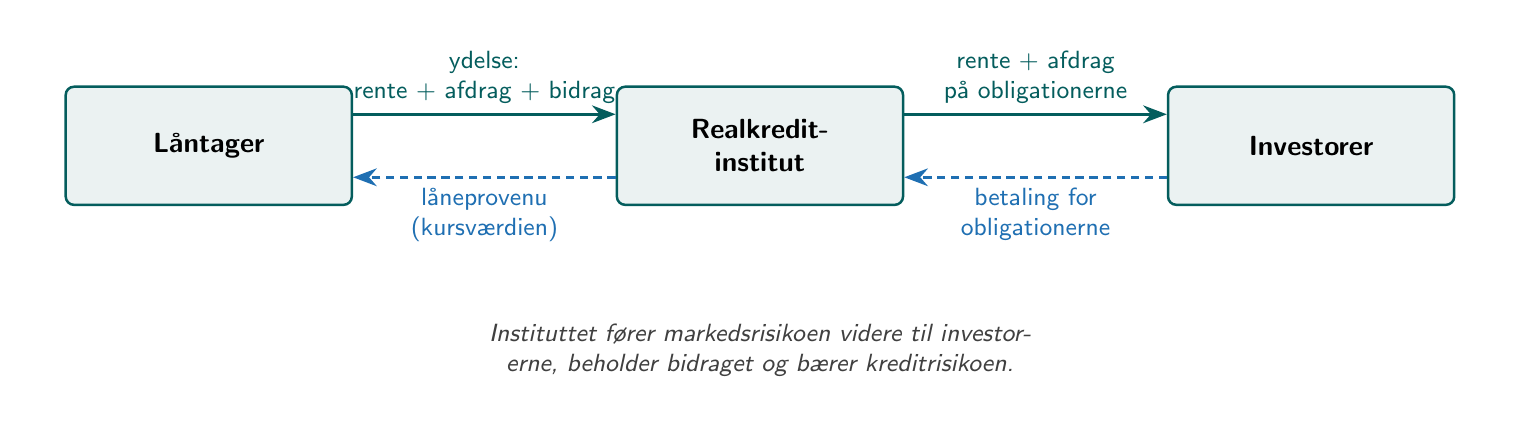
\begin{tikzpicture}[
    part/.style   = {draw=brandteal, line width=0.9pt, rounded corners=3pt,
                     fill=brandteal!8, align=center, minimum height=15mm,
                     text width=34mm, font=\normalsize\bfseries},
    lblup/.style  = {font=\small, align=center, text width=38mm, text=flowout},
    lbldn/.style  = {font=\small, align=center, text width=38mm, text=flowin},
    servicing/.style = {-{Stealth[length=3mm]}, line width=1.1pt, flowout},
    origin/.style    = {-{Stealth[length=3mm]}, line width=1.1pt, flowin, densely dashed},
]

% Fixed canvas so every phase exports at identical size -> the reveal.js
% fragment-stack animates without the boxes jumping between steps.
\useasboundingbox (-2.3,-3.4) rectangle (16.3,1.5);

% --- the three parties -------------------------------------------------
\node[part] (laantager) at (0,0)   {Låntager};
\node[part] (institut)  at (7,0)   {Realkredit-\\institut};
\node[part] (investor)  at (14,0)  {Investorer};

% --- phase 1: origination (money flows in, bottom arrows) --------------
\ifnum\phase>0
  \draw[origin] ([yshift=-4mm]investor.west) --
        node[lbldn, below] {betaling for\\obligationerne}
        ([yshift=-4mm]institut.east);
  \draw[origin] ([yshift=-4mm]institut.west) --
        node[lbldn, below] {låneprovenu\\(kursværdien)}
        ([yshift=-4mm]laantager.east);
\fi

% --- phase 2: servicing (life of the loan, top arrows) ----------------
\ifnum\phase>1
  \draw[servicing] ([yshift=4mm]laantager.east) --
        node[lblup, above] {ydelse:\\rente + afdrag + bidrag}
        ([yshift=4mm]institut.west);
  \draw[servicing] ([yshift=4mm]institut.east) --
        node[lblup, above] {rente + afdrag\\på obligationerne}
        ([yshift=4mm]investor.west);
  \node[align=center, font=\small\itshape, text width=105mm, text=black!75]
        at (7,-2.6)
        {Instituttet fører markedsrisikoen videre til investorerne,
         beholder bidraget og bærer kreditrisikoen.};
\fi

\end{tikzpicture}
\end{document}
"
%  then dvisvgm --pdf on each. See build_tikz.sh in this folder.
% =====================================================================
\providecommand{\phase}{2}      % default: full figure
\documentclass[border=6pt]{standalone}
\usepackage[T1]{fontenc}
\usepackage[utf8]{inputenc}
\usepackage[scaled=0.98]{helvet}
\renewcommand{\familydefault}{\sfdefault}
\usepackage{tikz}
\usetikzlibrary{arrows.meta, positioning, calc}

\definecolor{brandteal}{HTML}{045D5D}
\definecolor{brandgold}{HTML}{C9A227} % muted gold (readable on white)
\definecolor{flowin}{HTML}{1F6FB2}    % origination flow (blue)
\definecolor{flowout}{HTML}{045D5D}   % servicing flow (teal)

\begin{document}
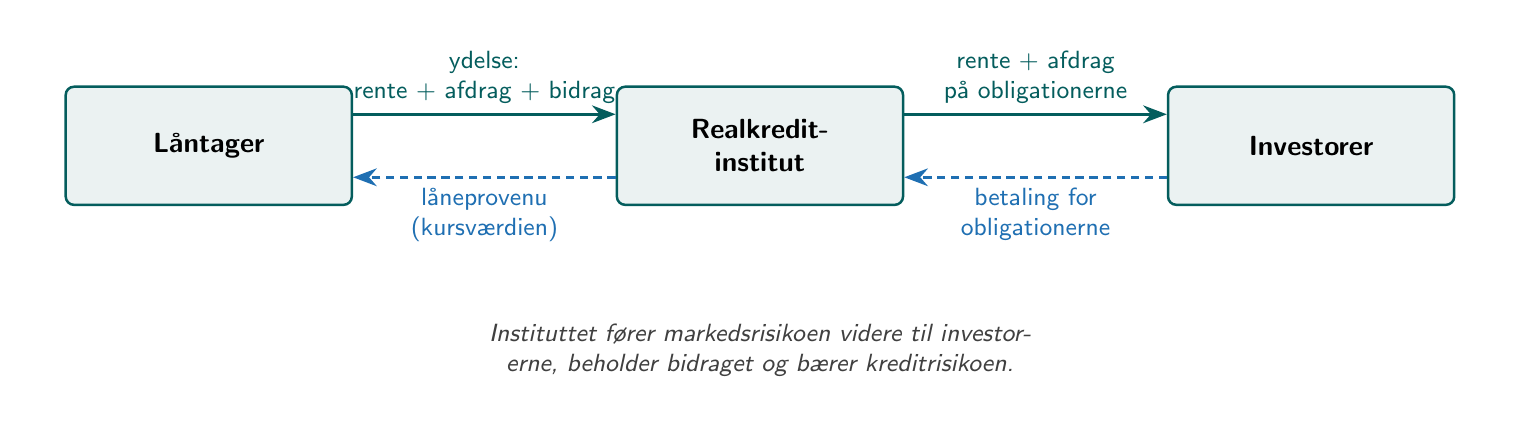
\begin{tikzpicture}[
    part/.style   = {draw=brandteal, line width=0.9pt, rounded corners=3pt,
                     fill=brandteal!8, align=center, minimum height=15mm,
                     text width=34mm, font=\normalsize\bfseries},
    lblup/.style  = {font=\small, align=center, text width=38mm, text=flowout},
    lbldn/.style  = {font=\small, align=center, text width=38mm, text=flowin},
    servicing/.style = {-{Stealth[length=3mm]}, line width=1.1pt, flowout},
    origin/.style    = {-{Stealth[length=3mm]}, line width=1.1pt, flowin, densely dashed},
]

% Fixed canvas so every phase exports at identical size -> the reveal.js
% fragment-stack animates without the boxes jumping between steps.
\useasboundingbox (-2.3,-3.4) rectangle (16.3,1.5);

% --- the three parties -------------------------------------------------
\node[part] (laantager) at (0,0)   {Låntager};
\node[part] (institut)  at (7,0)   {Realkredit-\\institut};
\node[part] (investor)  at (14,0)  {Investorer};

% --- phase 1: origination (money flows in, bottom arrows) --------------
\ifnum\phase>0
  \draw[origin] ([yshift=-4mm]investor.west) --
        node[lbldn, below] {betaling for\\obligationerne}
        ([yshift=-4mm]institut.east);
  \draw[origin] ([yshift=-4mm]institut.west) --
        node[lbldn, below] {låneprovenu\\(kursværdien)}
        ([yshift=-4mm]laantager.east);
\fi

% --- phase 2: servicing (life of the loan, top arrows) ----------------
\ifnum\phase>1
  \draw[servicing] ([yshift=4mm]laantager.east) --
        node[lblup, above] {ydelse:\\rente + afdrag + bidrag}
        ([yshift=4mm]institut.west);
  \draw[servicing] ([yshift=4mm]institut.east) --
        node[lblup, above] {rente + afdrag\\på obligationerne}
        ([yshift=4mm]investor.west);
  \node[align=center, font=\small\itshape, text width=105mm, text=black!75]
        at (7,-2.6)
        {Instituttet fører markedsrisikoen videre til investorerne,
         beholder bidraget og bærer kreditrisikoen.};
\fi

\end{tikzpicture}
\end{document}
"  (rename out)
%     pdflatex "\def\phase{2}% =====================================================================
%  kap5_pengestroemme.tex  —  slide redraw of fig:kap5_pengestroemme
%  Source of truth: notes ch.5 "5 Realkredit.tex", figur pengestrømme.
%
%  Slide-optimised redraw (paper-density stripped, labels enlarged,
%  institut tinted in brand teal). Built in phases so the arrows can be
%  revealed one flow at a time on the slide (reveal.js fragment stack):
%     \phase = 1  ->  origination only  (money flows IN to fund the loan)
%     \phase = 2  ->  full              (+ servicing flows over the life)
%
%  Build (from slides_side/src/images/_tikz_src/):
%     pdflatex "\def\phase{1}% =====================================================================
%  kap5_pengestroemme.tex  —  slide redraw of fig:kap5_pengestroemme
%  Source of truth: notes ch.5 "5 Realkredit.tex", figur pengestrømme.
%
%  Slide-optimised redraw (paper-density stripped, labels enlarged,
%  institut tinted in brand teal). Built in phases so the arrows can be
%  revealed one flow at a time on the slide (reveal.js fragment stack):
%     \phase = 1  ->  origination only  (money flows IN to fund the loan)
%     \phase = 2  ->  full              (+ servicing flows over the life)
%
%  Build (from slides_side/src/images/_tikz_src/):
%     pdflatex "\def\phase{1}\input{kap5_pengestroemme.tex}"  (rename out)
%     pdflatex "\def\phase{2}\input{kap5_pengestroemme.tex}"
%  then dvisvgm --pdf on each. See build_tikz.sh in this folder.
% =====================================================================
\providecommand{\phase}{2}      % default: full figure
\documentclass[border=6pt]{standalone}
\usepackage[T1]{fontenc}
\usepackage[utf8]{inputenc}
\usepackage[scaled=0.98]{helvet}
\renewcommand{\familydefault}{\sfdefault}
\usepackage{tikz}
\usetikzlibrary{arrows.meta, positioning, calc}

\definecolor{brandteal}{HTML}{045D5D}
\definecolor{brandgold}{HTML}{C9A227} % muted gold (readable on white)
\definecolor{flowin}{HTML}{1F6FB2}    % origination flow (blue)
\definecolor{flowout}{HTML}{045D5D}   % servicing flow (teal)

\begin{document}
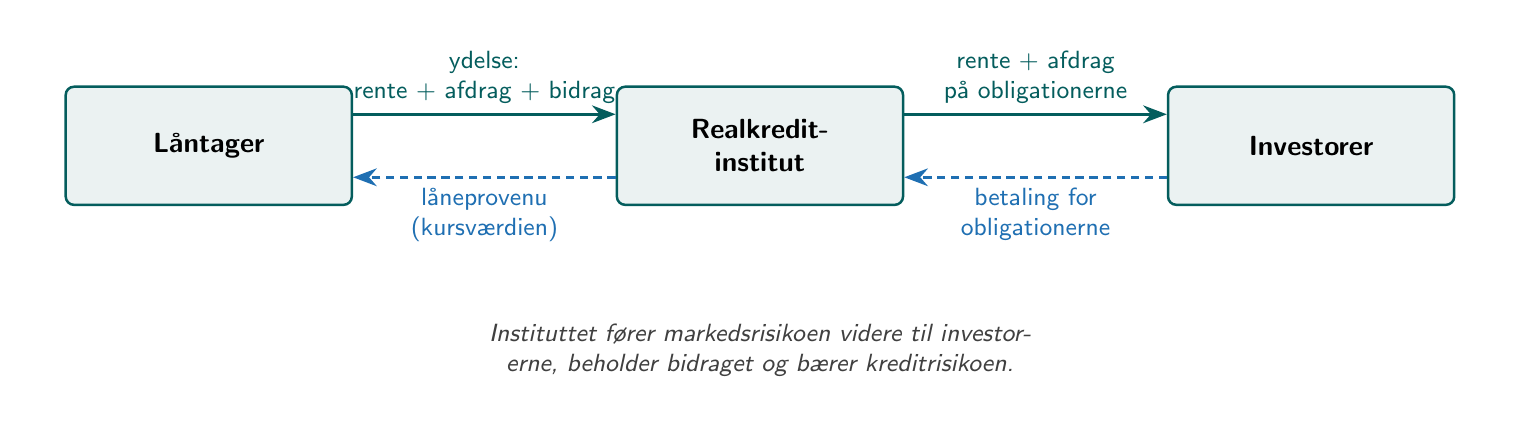
\begin{tikzpicture}[
    part/.style   = {draw=brandteal, line width=0.9pt, rounded corners=3pt,
                     fill=brandteal!8, align=center, minimum height=15mm,
                     text width=34mm, font=\normalsize\bfseries},
    lblup/.style  = {font=\small, align=center, text width=38mm, text=flowout},
    lbldn/.style  = {font=\small, align=center, text width=38mm, text=flowin},
    servicing/.style = {-{Stealth[length=3mm]}, line width=1.1pt, flowout},
    origin/.style    = {-{Stealth[length=3mm]}, line width=1.1pt, flowin, densely dashed},
]

% Fixed canvas so every phase exports at identical size -> the reveal.js
% fragment-stack animates without the boxes jumping between steps.
\useasboundingbox (-2.3,-3.4) rectangle (16.3,1.5);

% --- the three parties -------------------------------------------------
\node[part] (laantager) at (0,0)   {Låntager};
\node[part] (institut)  at (7,0)   {Realkredit-\\institut};
\node[part] (investor)  at (14,0)  {Investorer};

% --- phase 1: origination (money flows in, bottom arrows) --------------
\ifnum\phase>0
  \draw[origin] ([yshift=-4mm]investor.west) --
        node[lbldn, below] {betaling for\\obligationerne}
        ([yshift=-4mm]institut.east);
  \draw[origin] ([yshift=-4mm]institut.west) --
        node[lbldn, below] {låneprovenu\\(kursværdien)}
        ([yshift=-4mm]laantager.east);
\fi

% --- phase 2: servicing (life of the loan, top arrows) ----------------
\ifnum\phase>1
  \draw[servicing] ([yshift=4mm]laantager.east) --
        node[lblup, above] {ydelse:\\rente + afdrag + bidrag}
        ([yshift=4mm]institut.west);
  \draw[servicing] ([yshift=4mm]institut.east) --
        node[lblup, above] {rente + afdrag\\på obligationerne}
        ([yshift=4mm]investor.west);
  \node[align=center, font=\small\itshape, text width=105mm, text=black!75]
        at (7,-2.6)
        {Instituttet fører markedsrisikoen videre til investorerne,
         beholder bidraget og bærer kreditrisikoen.};
\fi

\end{tikzpicture}
\end{document}
"  (rename out)
%     pdflatex "\def\phase{2}% =====================================================================
%  kap5_pengestroemme.tex  —  slide redraw of fig:kap5_pengestroemme
%  Source of truth: notes ch.5 "5 Realkredit.tex", figur pengestrømme.
%
%  Slide-optimised redraw (paper-density stripped, labels enlarged,
%  institut tinted in brand teal). Built in phases so the arrows can be
%  revealed one flow at a time on the slide (reveal.js fragment stack):
%     \phase = 1  ->  origination only  (money flows IN to fund the loan)
%     \phase = 2  ->  full              (+ servicing flows over the life)
%
%  Build (from slides_side/src/images/_tikz_src/):
%     pdflatex "\def\phase{1}\input{kap5_pengestroemme.tex}"  (rename out)
%     pdflatex "\def\phase{2}\input{kap5_pengestroemme.tex}"
%  then dvisvgm --pdf on each. See build_tikz.sh in this folder.
% =====================================================================
\providecommand{\phase}{2}      % default: full figure
\documentclass[border=6pt]{standalone}
\usepackage[T1]{fontenc}
\usepackage[utf8]{inputenc}
\usepackage[scaled=0.98]{helvet}
\renewcommand{\familydefault}{\sfdefault}
\usepackage{tikz}
\usetikzlibrary{arrows.meta, positioning, calc}

\definecolor{brandteal}{HTML}{045D5D}
\definecolor{brandgold}{HTML}{C9A227} % muted gold (readable on white)
\definecolor{flowin}{HTML}{1F6FB2}    % origination flow (blue)
\definecolor{flowout}{HTML}{045D5D}   % servicing flow (teal)

\begin{document}
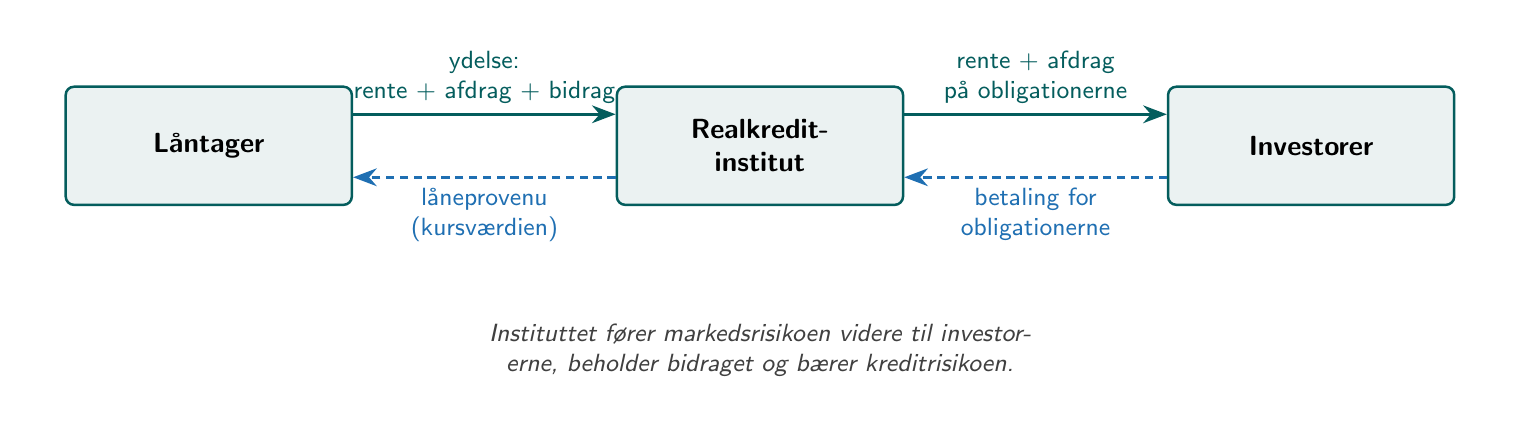
\begin{tikzpicture}[
    part/.style   = {draw=brandteal, line width=0.9pt, rounded corners=3pt,
                     fill=brandteal!8, align=center, minimum height=15mm,
                     text width=34mm, font=\normalsize\bfseries},
    lblup/.style  = {font=\small, align=center, text width=38mm, text=flowout},
    lbldn/.style  = {font=\small, align=center, text width=38mm, text=flowin},
    servicing/.style = {-{Stealth[length=3mm]}, line width=1.1pt, flowout},
    origin/.style    = {-{Stealth[length=3mm]}, line width=1.1pt, flowin, densely dashed},
]

% Fixed canvas so every phase exports at identical size -> the reveal.js
% fragment-stack animates without the boxes jumping between steps.
\useasboundingbox (-2.3,-3.4) rectangle (16.3,1.5);

% --- the three parties -------------------------------------------------
\node[part] (laantager) at (0,0)   {Låntager};
\node[part] (institut)  at (7,0)   {Realkredit-\\institut};
\node[part] (investor)  at (14,0)  {Investorer};

% --- phase 1: origination (money flows in, bottom arrows) --------------
\ifnum\phase>0
  \draw[origin] ([yshift=-4mm]investor.west) --
        node[lbldn, below] {betaling for\\obligationerne}
        ([yshift=-4mm]institut.east);
  \draw[origin] ([yshift=-4mm]institut.west) --
        node[lbldn, below] {låneprovenu\\(kursværdien)}
        ([yshift=-4mm]laantager.east);
\fi

% --- phase 2: servicing (life of the loan, top arrows) ----------------
\ifnum\phase>1
  \draw[servicing] ([yshift=4mm]laantager.east) --
        node[lblup, above] {ydelse:\\rente + afdrag + bidrag}
        ([yshift=4mm]institut.west);
  \draw[servicing] ([yshift=4mm]institut.east) --
        node[lblup, above] {rente + afdrag\\på obligationerne}
        ([yshift=4mm]investor.west);
  \node[align=center, font=\small\itshape, text width=105mm, text=black!75]
        at (7,-2.6)
        {Instituttet fører markedsrisikoen videre til investorerne,
         beholder bidraget og bærer kreditrisikoen.};
\fi

\end{tikzpicture}
\end{document}
"
%  then dvisvgm --pdf on each. See build_tikz.sh in this folder.
% =====================================================================
\providecommand{\phase}{2}      % default: full figure
\documentclass[border=6pt]{standalone}
\usepackage[T1]{fontenc}
\usepackage[utf8]{inputenc}
\usepackage[scaled=0.98]{helvet}
\renewcommand{\familydefault}{\sfdefault}
\usepackage{tikz}
\usetikzlibrary{arrows.meta, positioning, calc}

\definecolor{brandteal}{HTML}{045D5D}
\definecolor{brandgold}{HTML}{C9A227} % muted gold (readable on white)
\definecolor{flowin}{HTML}{1F6FB2}    % origination flow (blue)
\definecolor{flowout}{HTML}{045D5D}   % servicing flow (teal)

\begin{document}
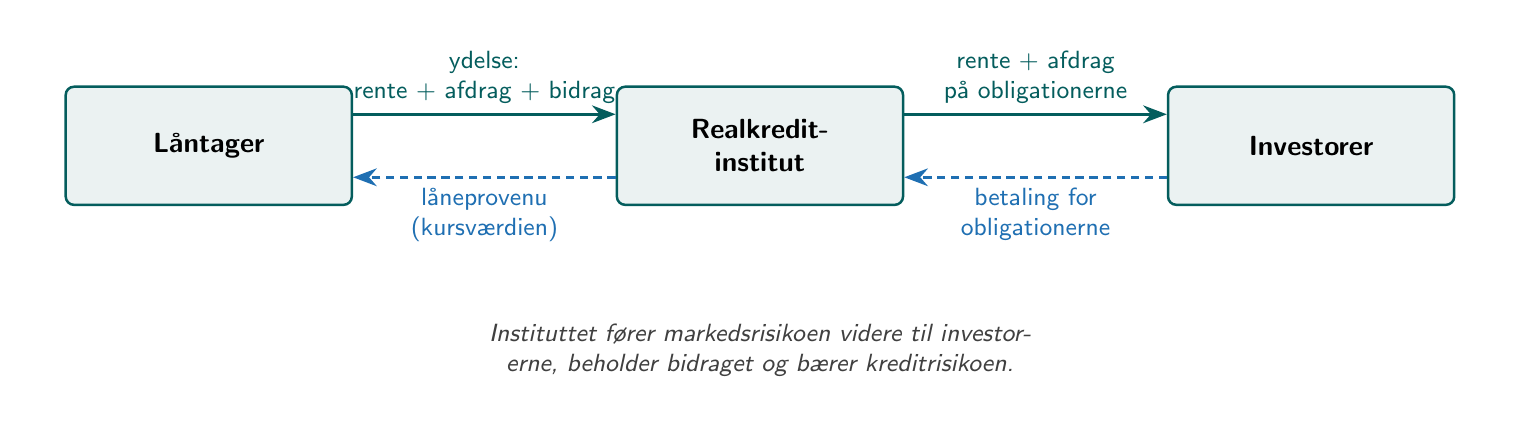
\begin{tikzpicture}[
    part/.style   = {draw=brandteal, line width=0.9pt, rounded corners=3pt,
                     fill=brandteal!8, align=center, minimum height=15mm,
                     text width=34mm, font=\normalsize\bfseries},
    lblup/.style  = {font=\small, align=center, text width=38mm, text=flowout},
    lbldn/.style  = {font=\small, align=center, text width=38mm, text=flowin},
    servicing/.style = {-{Stealth[length=3mm]}, line width=1.1pt, flowout},
    origin/.style    = {-{Stealth[length=3mm]}, line width=1.1pt, flowin, densely dashed},
]

% Fixed canvas so every phase exports at identical size -> the reveal.js
% fragment-stack animates without the boxes jumping between steps.
\useasboundingbox (-2.3,-3.4) rectangle (16.3,1.5);

% --- the three parties -------------------------------------------------
\node[part] (laantager) at (0,0)   {Låntager};
\node[part] (institut)  at (7,0)   {Realkredit-\\institut};
\node[part] (investor)  at (14,0)  {Investorer};

% --- phase 1: origination (money flows in, bottom arrows) --------------
\ifnum\phase>0
  \draw[origin] ([yshift=-4mm]investor.west) --
        node[lbldn, below] {betaling for\\obligationerne}
        ([yshift=-4mm]institut.east);
  \draw[origin] ([yshift=-4mm]institut.west) --
        node[lbldn, below] {låneprovenu\\(kursværdien)}
        ([yshift=-4mm]laantager.east);
\fi

% --- phase 2: servicing (life of the loan, top arrows) ----------------
\ifnum\phase>1
  \draw[servicing] ([yshift=4mm]laantager.east) --
        node[lblup, above] {ydelse:\\rente + afdrag + bidrag}
        ([yshift=4mm]institut.west);
  \draw[servicing] ([yshift=4mm]institut.east) --
        node[lblup, above] {rente + afdrag\\på obligationerne}
        ([yshift=4mm]investor.west);
  \node[align=center, font=\small\itshape, text width=105mm, text=black!75]
        at (7,-2.6)
        {Instituttet fører markedsrisikoen videre til investorerne,
         beholder bidraget og bærer kreditrisikoen.};
\fi

\end{tikzpicture}
\end{document}
"
%  then dvisvgm --pdf on each. See build_tikz.sh in this folder.
% =====================================================================
\providecommand{\phase}{2}      % default: full figure
\documentclass[border=6pt]{standalone}
\usepackage[T1]{fontenc}
\usepackage[utf8]{inputenc}
\usepackage[scaled=0.98]{helvet}
\renewcommand{\familydefault}{\sfdefault}
\usepackage{tikz}
\usetikzlibrary{arrows.meta, positioning, calc}

\definecolor{brandteal}{HTML}{045D5D}
\definecolor{brandgold}{HTML}{C9A227} % muted gold (readable on white)
\definecolor{flowin}{HTML}{1F6FB2}    % origination flow (blue)
\definecolor{flowout}{HTML}{045D5D}   % servicing flow (teal)

\begin{document}
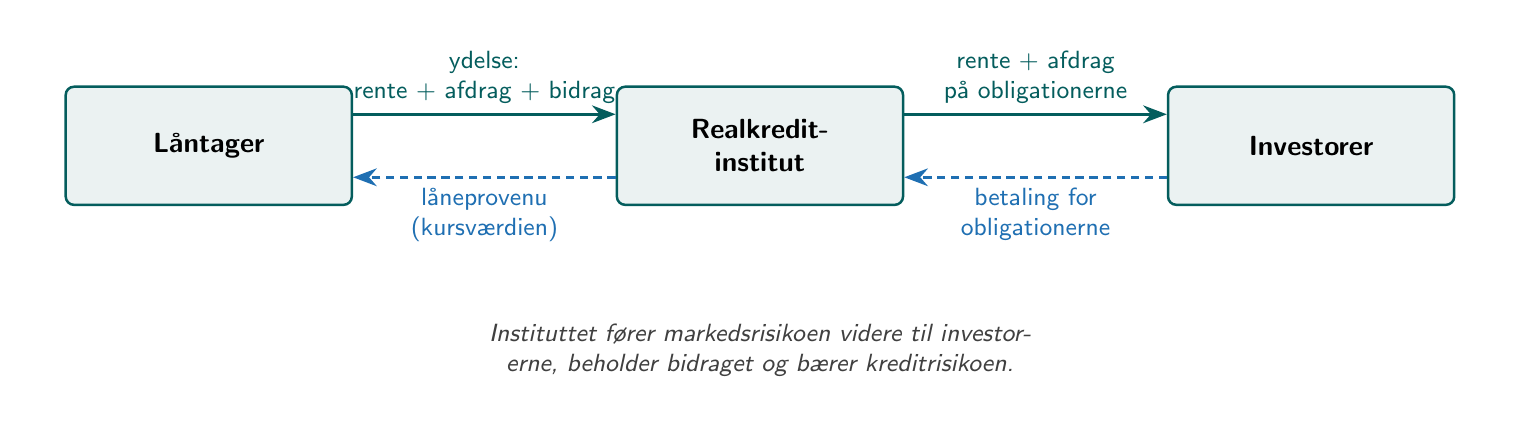
\begin{tikzpicture}[
    part/.style   = {draw=brandteal, line width=0.9pt, rounded corners=3pt,
                     fill=brandteal!8, align=center, minimum height=15mm,
                     text width=34mm, font=\normalsize\bfseries},
    lblup/.style  = {font=\small, align=center, text width=38mm, text=flowout},
    lbldn/.style  = {font=\small, align=center, text width=38mm, text=flowin},
    servicing/.style = {-{Stealth[length=3mm]}, line width=1.1pt, flowout},
    origin/.style    = {-{Stealth[length=3mm]}, line width=1.1pt, flowin, densely dashed},
]

% Fixed canvas so every phase exports at identical size -> the reveal.js
% fragment-stack animates without the boxes jumping between steps.
\useasboundingbox (-2.3,-3.4) rectangle (16.3,1.5);

% --- the three parties -------------------------------------------------
\node[part] (laantager) at (0,0)   {Låntager};
\node[part] (institut)  at (7,0)   {Realkredit-\\institut};
\node[part] (investor)  at (14,0)  {Investorer};

% --- phase 1: origination (money flows in, bottom arrows) --------------
\ifnum\phase>0
  \draw[origin] ([yshift=-4mm]investor.west) --
        node[lbldn, below] {betaling for\\obligationerne}
        ([yshift=-4mm]institut.east);
  \draw[origin] ([yshift=-4mm]institut.west) --
        node[lbldn, below] {låneprovenu\\(kursværdien)}
        ([yshift=-4mm]laantager.east);
\fi

% --- phase 2: servicing (life of the loan, top arrows) ----------------
\ifnum\phase>1
  \draw[servicing] ([yshift=4mm]laantager.east) --
        node[lblup, above] {ydelse:\\rente + afdrag + bidrag}
        ([yshift=4mm]institut.west);
  \draw[servicing] ([yshift=4mm]institut.east) --
        node[lblup, above] {rente + afdrag\\på obligationerne}
        ([yshift=4mm]investor.west);
  \node[align=center, font=\small\itshape, text width=105mm, text=black!75]
        at (7,-2.6)
        {Instituttet fører markedsrisikoen videre til investorerne,
         beholder bidraget og bærer kreditrisikoen.};
\fi

\end{tikzpicture}
\end{document}
"
%  then dvisvgm --pdf on each. See build_tikz.sh in this folder.
% =====================================================================
\providecommand{\phase}{2}      % default: full figure
\documentclass[border=6pt]{standalone}
\usepackage[T1]{fontenc}
\usepackage[utf8]{inputenc}
\usepackage[scaled=0.98]{helvet}
\renewcommand{\familydefault}{\sfdefault}
\usepackage{tikz}
\usetikzlibrary{arrows.meta, positioning, calc}

\definecolor{brandteal}{HTML}{045D5D}
\definecolor{brandgold}{HTML}{C9A227} % muted gold (readable on white)
\definecolor{flowin}{HTML}{1F6FB2}    % origination flow (blue)
\definecolor{flowout}{HTML}{045D5D}   % servicing flow (teal)

\begin{document}
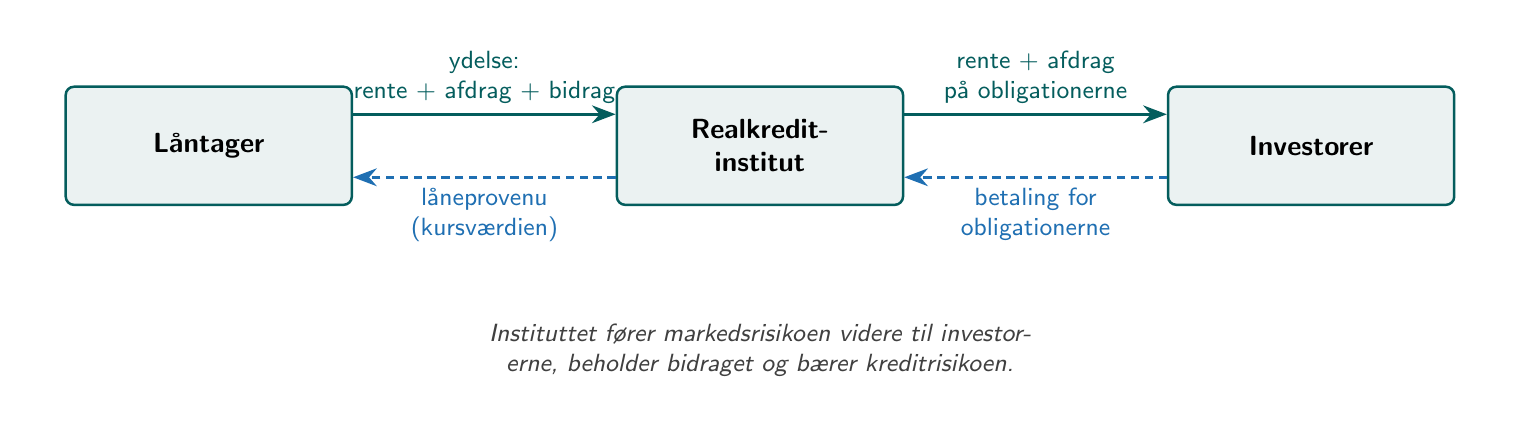
\begin{tikzpicture}[
    part/.style   = {draw=brandteal, line width=0.9pt, rounded corners=3pt,
                     fill=brandteal!8, align=center, minimum height=15mm,
                     text width=34mm, font=\normalsize\bfseries},
    lblup/.style  = {font=\small, align=center, text width=38mm, text=flowout},
    lbldn/.style  = {font=\small, align=center, text width=38mm, text=flowin},
    servicing/.style = {-{Stealth[length=3mm]}, line width=1.1pt, flowout},
    origin/.style    = {-{Stealth[length=3mm]}, line width=1.1pt, flowin, densely dashed},
]

% Fixed canvas so every phase exports at identical size -> the reveal.js
% fragment-stack animates without the boxes jumping between steps.
\useasboundingbox (-2.3,-3.4) rectangle (16.3,1.5);

% --- the three parties -------------------------------------------------
\node[part] (laantager) at (0,0)   {Låntager};
\node[part] (institut)  at (7,0)   {Realkredit-\\institut};
\node[part] (investor)  at (14,0)  {Investorer};

% --- phase 1: origination (money flows in, bottom arrows) --------------
\ifnum\phase>0
  \draw[origin] ([yshift=-4mm]investor.west) --
        node[lbldn, below] {betaling for\\obligationerne}
        ([yshift=-4mm]institut.east);
  \draw[origin] ([yshift=-4mm]institut.west) --
        node[lbldn, below] {låneprovenu\\(kursværdien)}
        ([yshift=-4mm]laantager.east);
\fi

% --- phase 2: servicing (life of the loan, top arrows) ----------------
\ifnum\phase>1
  \draw[servicing] ([yshift=4mm]laantager.east) --
        node[lblup, above] {ydelse:\\rente + afdrag + bidrag}
        ([yshift=4mm]institut.west);
  \draw[servicing] ([yshift=4mm]institut.east) --
        node[lblup, above] {rente + afdrag\\på obligationerne}
        ([yshift=4mm]investor.west);
  \node[align=center, font=\small\itshape, text width=105mm, text=black!75]
        at (7,-2.6)
        {Instituttet fører markedsrisikoen videre til investorerne,
         beholder bidraget og bærer kreditrisikoen.};
\fi

\end{tikzpicture}
\end{document}
